\section{Usability-Analyse}

\begin{frame}
	\begin{center}
		\huge{Usability-Analyse}
	\end{center}
\end{frame}

\begin{frame}
	\frametitle{Vorgehensweise}
	\begin{itemize}
		\item[1] Grobe Seitenauswahl 
		\item[2] Fragebogen ausfüllen
		\item[3] Fazit pro Seite
		\item[4] Stetige Re-Evaluation während Implementierung
	\end{itemize}
\end{frame}

\begin{frame}
	\frametitle{Usability Analyse}
	Basierend auf der Idee werden Konkurrenten bestimmt
	\begin{itemize}
		\item Absolut Vodka
		\item Alnatura
		\item Bacardi
		\item Fritz Kola
		\item Mate Drinks
		\item MyMuesli
	\end{itemize}
\end{frame}


\subsection{Positiv Beispiel}
\begin{frame}
	\frametitle{Beispiel Absolut I}
	\begin{figure}
	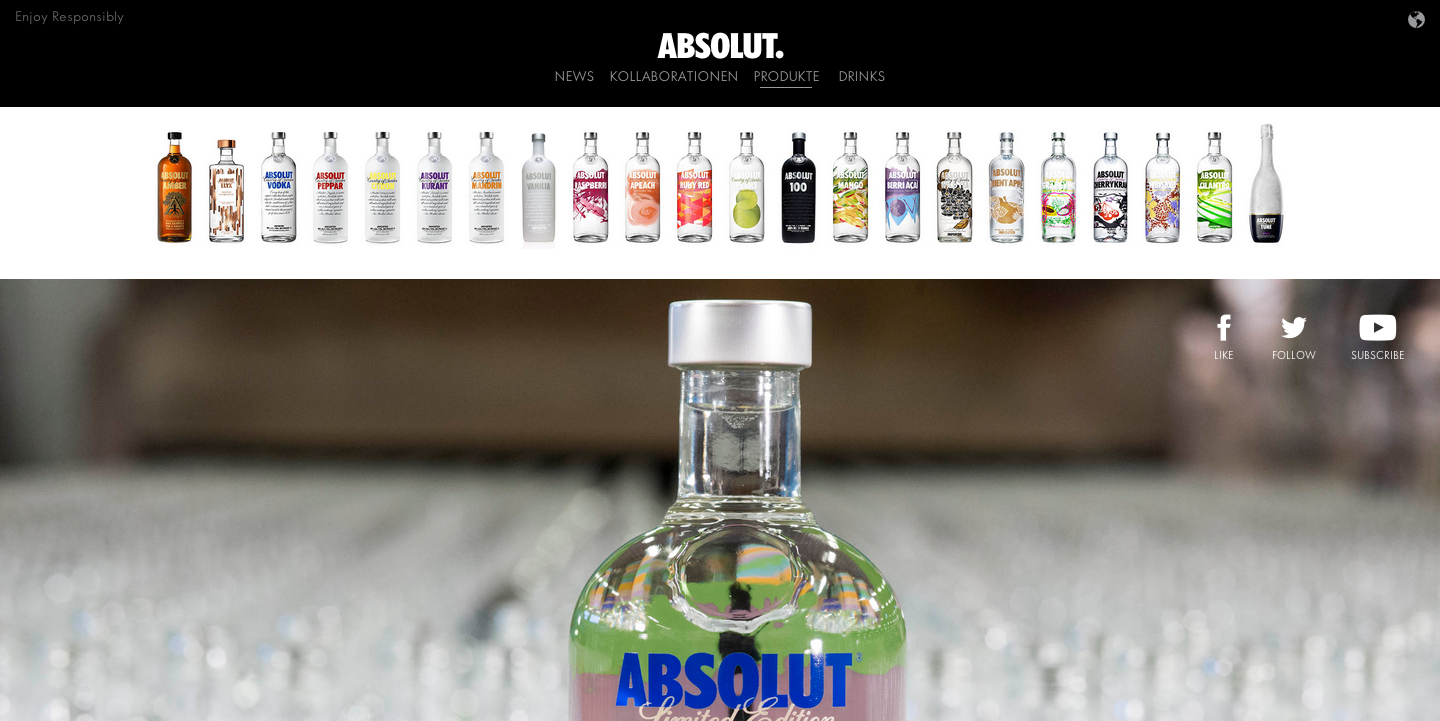
\includegraphics[scale=0.2]{bilder/absolut.png}
	\label{labelname}
	\end{figure}
\end{frame}

\begin{frame}
	\frametitle{Beispiel Absolut II}
	\begin{tabular}{|p{2,4cm}|l|p{6cm}|}
	\hline
	  Kriterium & Punkte & Kommentar \\ \hline
  	  Aktualität & 9 & Blog mit aktuellen (nicht täglich) Einträgen; aktuelle Produktlinie \\ \hline
	  (Benutzer-) Sicherheit & 7 & Keine Speicherung Benutzerbezogener Daten; Cookies; Nutzungsverhalten wird gespeichert (Häufigkeit, Dauer...); Angeblich werden Standardschutzmaßnahmen eingesetzt \\ \hline
	  Beschreibung der Informationen & 10 & Sehr wenige Ebenen; kompakte und dennoch präzise Navigation anhand treffender Stichworte \\ \hline
 	\end{tabular}
\end{frame}

\begin{frame}
	\frametitle{Beispiel Absolut III}
	\begin{tabular}{|p{2,4cm}|l|p{6cm}|}
	\hline
	  Kriterium & Punkte & Kommentar \\ \hline
	  Qualität der Daten & 9 & Produkte werden sehr genau beschrieben, nicht nur im Bezug auf das Endprodukt, sondern auch Herkunft der Ausgangsmaterialien und Fertigungsprozess \\ \hline
	  UI, Erwartungshaltung, altersgerecht, etc. & 8 & Drinkrezeptsuche; UI sehr übersichtlich und intuitiv (dauernd eingeblendete Navi-Leiste oben), sowie passend für Zielgruppe; Erwartungshaltung übertroffen (Es werden Rezepte bereitgestellt... auch für anderen Alkohol, sowie ein Blog mit aktuellen Themen rund um die Marke) \\ \hline
 	\end{tabular}
\end{frame}

\begin{frame}
	\frametitle{Beispiel Absolut IV}
	\begin{tabular}{|p{2,4cm}|l|p{6cm}|}
	\hline
	  Kriterium & Punkte & Kommentar \\ \hline
	  Fremdsprachen & 8 & Große Mengen an Fremdsprachen; kleinere Fehler \\ \hline
	  Volltextdaten & 10 & Nahezu nur Volltextdaten; Stichwortartige Daten bei passenden Gelegenheiten (Rezepte) \\ \hline
	  Druckunter- Stützung & 0 & Nicht vorhanden \\ \hline
	  Vielfältigkeit & 10 & Hohe Vielfalt; Angebot übertrifft der einfachen Präsentation der angebotenen Produkte; Produkte werden nicht zentral abgebildet, sondern der Lifestyle von "Absolut Vodka"; Es werden Rezepte vorgeschlagen, sowie weltweite Events diskutiert \\ \hline
 	\end{tabular}
\end{frame}

\begin{frame}
	\frametitle{Beispiel Absolut V}
	\begin{tabular}{|p{2,4cm}|l|p{6cm}|}
	\hline
	  Dienstleistungs- treue, Ernsthaftigkeit des Providers & 10 & Sehr durchdachtes Konzept der Informationsdarbietung, welches sicherlich mit hohem Aufwand realisiert wurde; Wirkt sehr seriös; \\ \hline
 	\end{tabular}
\end{frame}

\begin{frame}\frametitle{Beispiel Absolut - Fazit}
	Aus den Betrachtungen sind Punkte abzuleiten, wie 
	\begin{itemize}
		\item Erwartungshaltung durch sekundäre Angebote übertreffen
		\item Simple Navigation
		\item Kundenbindung aufbauen
		\item Indirekte Informationsführung
	\end{itemize}
\end{frame}

\subsection{Negativ Beispiel}
\begin{frame}
	\frametitle{Beispiel Fritz-Kola}
	\begin{figure}
	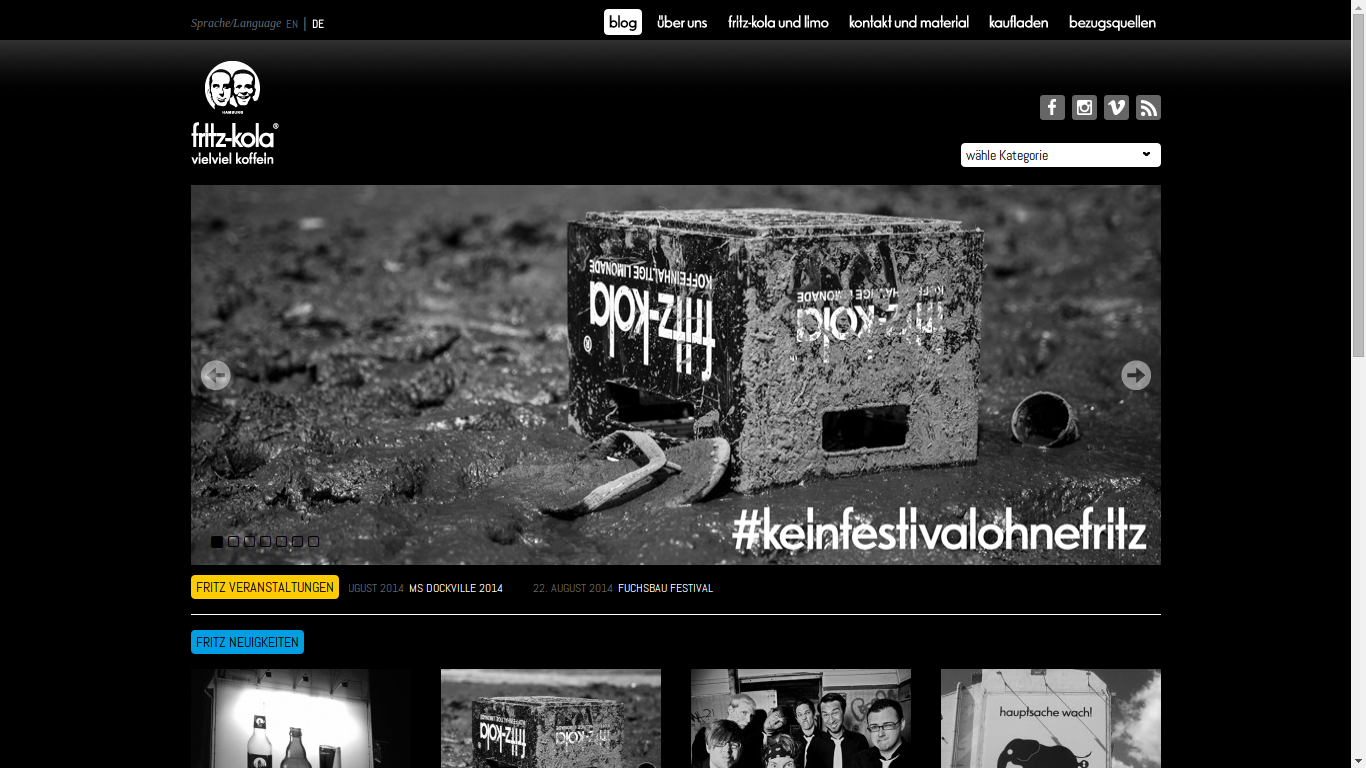
\includegraphics[scale=0.2]{bilder/fritz-kola.png}
	\end{figure}
\end{frame}

\begin{frame}
	\frametitle{Usability-Bogen (Auszug)}
	\begin{tabular}{|p{2,4cm}|l|p{6cm}|}
	  \hline
	  Kriterium & Punkte & Kommentar \\ \hline
	  Beschreibung der Informationen & 5 & Teils fehlende oder nichts-aussagende Überschriften bei News-Carousel.  \\ \hline	
	  
	  UI etc & 5 & Links im Fließtext nicht erkennbar. Redundante Filtermöglichkeiten. Tote Links. Unklare Navigationsstruktur. Keine Suche.  \\ \hline		
	  Fremdsprachen & 1 & Pseudo-Mehrsprachigkeit.  \\ \hline		
	\end{tabular}
\end{frame}

\begin{frame}
	\frametitle{Fritz-Kola Zusammenfassung}
	negativ:
	\begin{itemize}
		\item unhomogene Struktur
		\item Unklarheit bei Überschriften/Links
		\item Fehler
		\item Keine flache Navigationsstruktur
	\end{itemize}
	
	positiv:
	\begin{itemize}
		\item Inhaltsvielfalt
		\item Redaktionell gepflegt
		\item klare Zielgruppe
	\end{itemize}
\end{frame}

\subsection{Fazit}
\begin{frame}
	\frametitle{Unsere Erkenntnisse}
	Aus der Analyse entstandene Ziele (Auswahl)
	\begin{itemize}
		\item modernes übersichtliches Design % jede Seite sollte eigenen Charme haben.
		\item Flache Navigation
		\item Sinnvolle Suchfunktion % Tags
		\item Zum Wiederbesuch motivieren (Zielgruppeninteressen)
			\begin{itemize}
				\item Rezepte
				\item Veranstaltungen
				\item Blog
				\item persönliche Bindung zum Unternehmen wecken
			\end{itemize}
	\end{itemize}
\end{frame}

